\label{sec:DETRavenApproach}
RAVEN is able to perform DET analysis through the newly developed module ``\textbf{A}nalysis of \textbf{D}ynamic \textbf{R}eactor \textbf{A}ccident \textbf{E}volution'', that has been included in the RAVEN external Python manager.

Following the philosophy of the DET approach, this module lets RELAP-7 find the several possible outcomes of an accident sequence. When the system reaches certain conditions, for which more than one outcome may be possible (e.g. opening system of a valve damaged), a sampler generates the corresponding new set of branches (alternative sequences), associating a conditional probability to each.
\\The user defined branching laws can be based on the following logics:
\vspace{-5mm}
\begin{itemize}
\itemsep0em
\item Thresholds, either in terms of cumulative probability distribution or variable magnitude. An example is the failure of a pipe as a function of pressure probability distribution
\item On demand. An example is failure on demand of an actionable component (ie. relief valve)
\item Time driven. This is the simplest case where the user defines a branching logic, consequentially changing  the plant status, at a certain point in time
\end{itemize}
\vspace{-5mm}

For the analysis of complex systems, the number of branches may become extremely large. In order to avoid unacceptable growth of problem due by an excessive number of branches, the user needs to specify exit conditions for the simulation(termination laws). For example, maximum mission time, rules based on the simulator physical model (i.e. Maximum temperature of the fuel cladding, etc.).
\\In other similar codes, one of the most common termination laws is a probability cut-off: a branch's execution is stopped when its probability falls below a given limit.
%No countermeasures are generally taken to conserve the global probability.
This approach should be used with caution since it may have a large impact on the probability estimation of the possible final outcomes. This might happen when the number of branches is very large, and, therefore, the magnitude of their conditional probability is very low. In such a case, a large number of branches might be terminated before reaching the final outcome, biasing the analysis.  In order to avoid these issues and preserve the probability conservation, the user can not directly input, in RAVEN, a branching probability cut-off.
%As can be inferred from above, RAVEN provides capabilities to:
%\vspace{-5mm}
%\begin{itemize}
%\itemsep0em
%\item explore possible pathways through which the system can evolve
%\item quantify the probability of these scenarios
%\end{itemize}
%\vspace{-5mm}
%These main tasks are accomplished based on user specified branching and termination laws, %model of the system in RELAP-7, probability assignment rules to accident sequences (either by %inputed values or/and by distribution functions).
%The synergy among the different RAVEN modules gives to the package the flexibility to %summarize all the state of art DET capabilities.
%Indeed, as in similar tools~\cite{ADAPTHakobyan}, the DET module in RAVEN allows the user %use different approaches for defying the branching logic:
%\vspace{-5mm}
%\begin{itemize}
%\itemsep0em
%\item branching/failures on demand (i.e. time and field triggers)
%\item branching based on failure probability distributions
%\item multi-branching scenarios
%\end{itemize}
%\vspace{-5mm}
In RAVEN there is no distinction between the treatment of aleatory and epistemic variables. For example, the pressure at which a pipe fails to operate can be considered an epistemic variable, but it is treated the same as the recovery time of the auxiliary cooling system. Both variables can be handled with a branching logic driven by the associated CDFs or variables’ magnitude. The only case in which they might be treated differently is when an epistemic variable sets the initial value of a parameter. A classical example of this situation is the uncertainty associated to the parameters used in the RELAP-7 equations. Even in this case, it does not seem necessary to have a special treatment for these variables. In the DET module, this special case can be handled  with a multiple branch logic (two or more branches) at the begin of the initial simulation (ie. the simulation that represents the initiating event).

The above consideration, in conjunction with the brief overview of the mathematical framework analyzed in section~\ref{sec:mathFramework}, gives an indication on how RAVEN (and the DET module) combines all the capabilities present in other similar codes~\cite{ADAPTHakobyan}.
%In RAVEN there is no distinction between active (e.g. circulation pumps, valves, controlled %systems, etc.) and passive (e.g. steam generators, condensers, pipes, etc.) component %behaviors; all are treated as a aleatory uncertainties, since the physical conditions under which %a branching would occur for the them are determined by the thermal-hydraulic code RELAP-7 %without user ``control''. The user can model also the epistemic uncertainties, those due to lack %of knowledge of the phenomena analyzed (e.g. Heat capacity coefficient, etc.).
%In RAVEN, from an user point of view, both aleatory and epistemic uncertainties are %undifferentiated, since branching laws for either are specified in the same way. All triggers are %identified by their own PDFs and activated when an user defined probability threshold, on the %associated Cumulative Distribution Function (CDF), is exceeded.
%The probability thresholds on the CDFs are automatically handled by the DET module; the user %only needs to specify them in the input.

The user implements the DET logic in the \verb!Python! control logic input file, under the function named ``\emph{dynamic\_event\_tree}''. In this function, all the features available in RAVEN can be used (online monitoring, controlling, auxiliary system, probability distributions, utilities, etc.).
\begin{figure}[h]
  \centering
     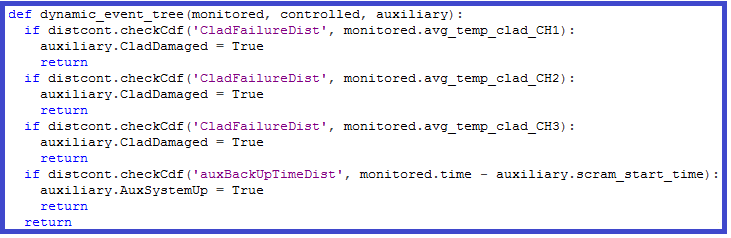
\includegraphics[width=0.8\textwidth]{figures/BranchingLaws.png}
  \caption{Example of DET logic}
   \label{fig:DET_branchLaws}
\end{figure}
\\As an example, Figure~\ref{fig:DET_branchLaws} lists set of branching rules. The ``checkCdf'' function, available in the distribution container, checks if the associated cumulative probability  threshold has been passed, and, if it has, sends a branching signal to RAVEN/RELAP-7 in order to print a restart file, that will be handled by the DET module.
%%%%%%%%%%%%%%%%%%%%%%%%%%%%%%
\subsection{Software Infrastructure}
\label{sec:CPUInfrastructure}
%%%%%%%%%%%%%%%%%%%%%%%%%%%%%%
In this section the software infrastructure for the DET generation is briefly presented. As already mentioned, the DET module is part of RAVEN's \verb!Python! external driver, which represents the core of PRA analysis.
\begin{figure}[h]
  \centering
     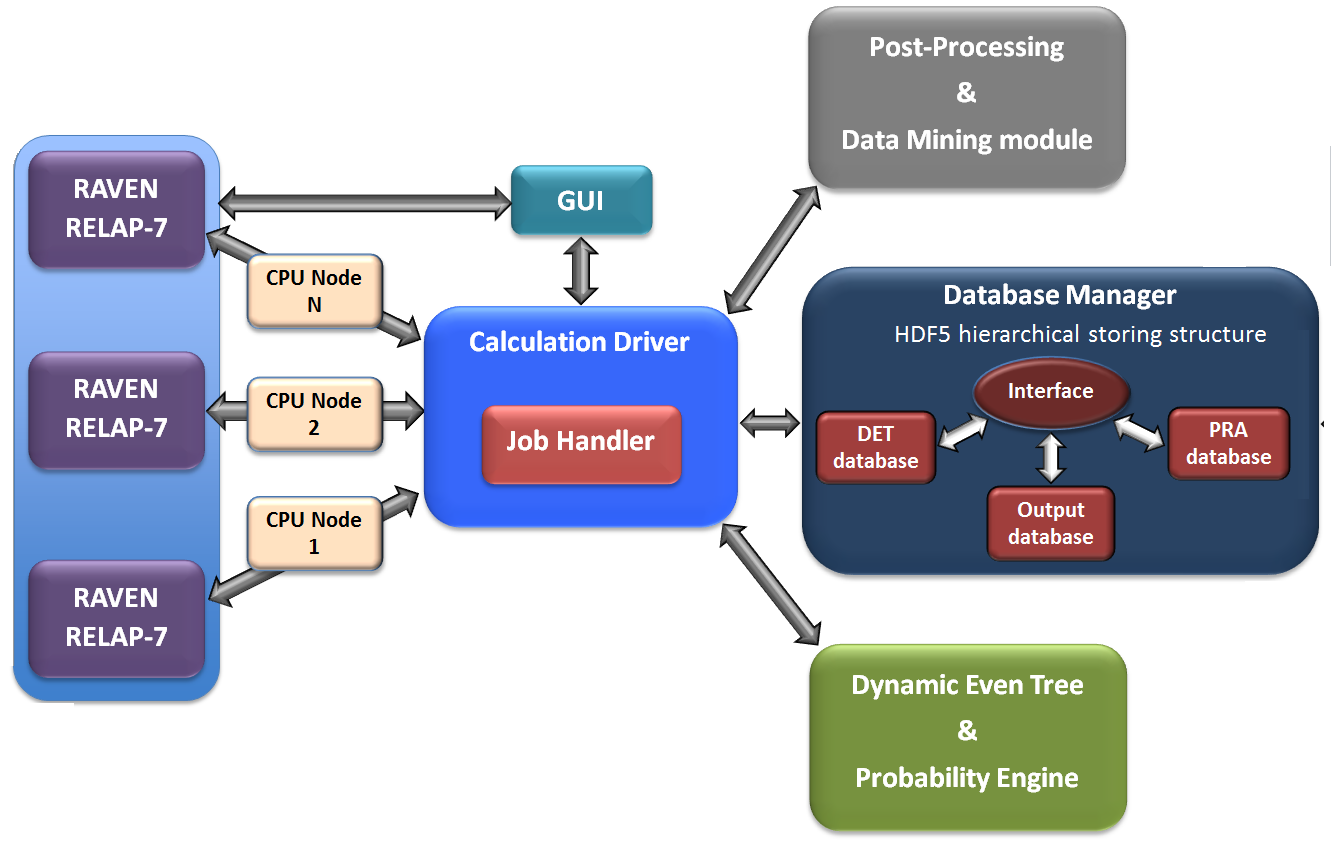
\includegraphics[width=0.70\textwidth]{figures/softwareCalcStructure.png}
  \caption{Software calculation infrastructure scheme}
   \label{fig:softwareInfrastructure}
\end{figure}

The external driver manager has the control of the different modules that support the DET calculation:
\vspace{-5mm}
\begin{itemize}
\itemsep0em
\item General Calculation Driver and Job Handler
\item Visualization and Input supporting GUI
\item DET and Probability Engine
\item Database manager
\item Post-processing and Data Mining module
\item Distributed Computing Environment Interface
\end{itemize}
\vspace{-5mm}
The General Calculation Driver is responsible to communicate information among the different modules. It is the only software branch that is aware of which modules are participating to the calculation.

Figure~\ref{fig:softwareInfrastructure} shows a schematic overview of the calculation structure, highlighting the most important modules that are involved in a DET calculation. Following an initiating event, the DET module provides initial conditions as well as the duration of the simulation (optionally) to the system simulator (i.e. RAVEN/RELAP-7).
\\The Calculation Driver, through the Job Handler module, runs the simulator until the control logic of RAVEN/RELAP-7 detects that a stopping condition is reached. The DET module decides whether to branch or not depending on the information received, through the general calculation driver, from RAVEN/RELAP-7.
The probability engine is in charge of computing the likelihood of branching generated by trigger signals (e.g. probability threshold on Clad Failure distribution exceeded).  If the DET module decides that $n$ branches are needed, it communicates to the Calculation Driver/Job Handler, that manages the jobs through a queue system, to execute the $n$ branches in $n$ different subprocesses (in parallel, if the machine is multi-processor, in sequence otherwise). The resulting tree structure, branch probabilities, trigger information, and simulation results are sent to the Database manager, that, based on the kind of information received, distributes the data among the sub-structures (DET, PRA, Output databases). The database manager is able to store data in different formats (e.g. HDF5, CSV, etc.).

The user can decide to perform post-processing operations and/or data mining manipulation on the fly, through the Post-processing and data mining module. The whole calculation may be visualized through the RAVEN GUI, that is able to exploit the communication capabilities present in the external calculation driver for following the simulation evolution (e.g. monitored variables or probability evolution through different branches, etc.). \\ The whole calculation infrastructure is designed to be agnostic regarding the machine in which it is running with extremely good performance either in PCs/workstations and HPC clusters.
